\documentclass{article}
\usepackage{tikz}
\usetikzlibrary{arrows.meta}

\begin{document}

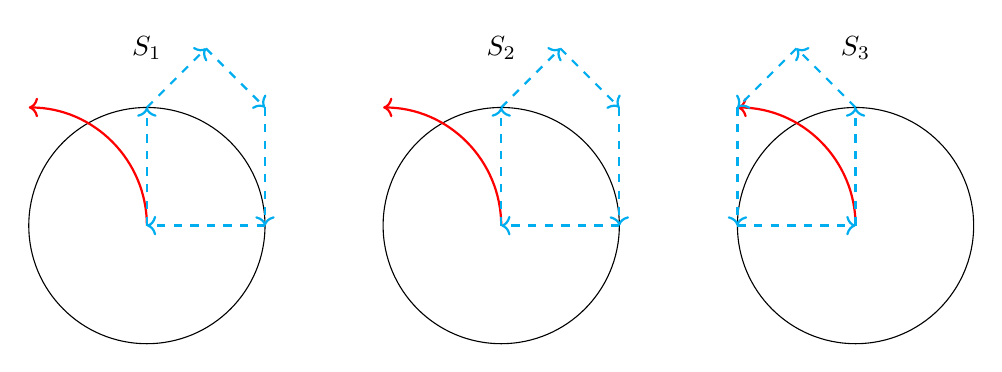
\begin{tikzpicture}[scale=1.5]
    % Draw circles
    \draw (0,0) circle (1);
    \draw (-3,0) circle (1);
    \draw (3,0) circle (1);

    % Label circles
    \node at (0,1.5) {$S_2$};
    \node at (-3,1.5) {$S_1$};
    \node at (3,1.5) {$S_3$};

    % Draw arrows
    \draw[->, red, thick] (0,0) arc (0:90:1);
    \draw[->, cyan, dashed, thick] (0,0) -- (0,1);
    \draw[->, cyan, dashed, thick] (0,1) -- (0.5,1.5);
    \draw[->, cyan, dashed, thick] (0.5,1.5) -- (1,1);
    \draw[->, cyan, dashed, thick] (1,1) -- (1,0);
    \draw[->, cyan, dashed, thick] (1,0) -- (0,0);

    \draw[->, red, thick] (-3,0) arc (0:90:1);
    \draw[->, cyan, dashed, thick] (-3,0) -- (-3,1);
    \draw[->, cyan, dashed, thick] (-3,1) -- (-2.5,1.5);
    \draw[->, cyan, dashed, thick] (-2.5,1.5) -- (-2,1);
    \draw[->, cyan, dashed, thick] (-2,1) -- (-2,0);
    \draw[->, cyan, dashed, thick] (-2,0) -- (-3,0);

    \draw[->, red, thick] (3,0) arc (0:90:1);
    \draw[->, cyan, dashed, thick] (3,0) -- (3,1);
    \draw[->, cyan, dashed, thick] (3,1) -- (2.5,1.5);
    \draw[->, cyan, dashed, thick] (2.5,1.5) -- (2,1);
    \draw[->, cyan, dashed, thick] (2,1) -- (2,0);
    \draw[->, cyan, dashed, thick] (2,0) -- (3,0);
\end{tikzpicture}

\end{document}